% chapter4 实验

\chapter{实验结果分析与模型评估}

\section{实验环境}

论文构建的HA-FuseNet是在实验室搭建的服务器上进行搭建和训练的,所用的软/硬件环境如表~\ref{tab:env}~所示:
\begin{table}[h]
    \centering
    \caption{实验环境}
    \label{tab:env}
    \begin{tabularx}{0.8\textwidth}{>{\centering\arraybackslash\hsize=0.6\hsize}X >{\centering\arraybackslash\hsize=1.4\hsize}X}
    \toprule
    软/硬件名称 & 型号/版本 \\
    \midrule
    操作系统 & Ubuntu 20.04.6 LTS  \\
    CPU & Intel(R) Xeon(R) Gold 5218R CPU @ 2.10GHz \\
    GPU & NVIDIA GeForce RTX 3090 \\
    内存 & 128GB \\
    显存 & 24GB \\
    CUDA & 11.8 \\
    Python & 3.11.5 \\
    Pytorch & 2.0.1 \\
    MNE & 1.6.0 \\
    Numpy & 1.26.3 \\
    \bottomrule
    \end{tabularx}
\end{table}

\section{数据与实验准备}

\subsection{运动想象脑电图数据集}

运动想象脑电图是使用脑电采集设备从头皮上获取的人类大脑的神经元活动时产生的生物电电位信号,能够反映大脑皮层和深层结构的功能状态及其异常变化。脑电图信号的采集过程主要包括以下几个步骤:

(1) 采集准备:根据国际10-20标准导联系统或其他标准定位方案,将电极安放在被试头皮的不同位置,以捕获不同脑区的电位信号。电极通常通过电极帽或电极盘固定,以确保位置的稳定和正确。由于人体脑电信号强度微弱,通常会通过与脑电采集设备相连的放大器对脑电信号进行增强和记录;

(2) 信号记录:当大脑神经元兴奋或抑制时,会产生微弱的电位变化,这些电位变化传导到头皮表面,形成可测量的电压差,由脑电采集系统进行捕获和放大。脑电采集系统通常以每秒进行\(N\)次连续采集的方式工作,即采集频率为\(N\)Hz;

(3) 数字化:根据脑电采集系统的设置,对被捕获的脑电信号进行一定的处理,包括通过模数转换器(Analog to Digital Converter,ADC)将模拟信号转换为数字信号。

在临床和科研应用中,脑电图信号因其非侵入性、实时监测性、对大脑功能活动的敏感性等特点,已经在大脑解码领域获得了广泛的应用。运动想象领域有多个公开的脑电图信号数据集,论文主要选取BCI Competition IV Dataset 2A\cite{brunner2008bci}数据集和BCI Competition IV Dataset 2B\cite{leeb2008bci}数据集作为模型训练和测试的数据集。BCI Competition(脑机接口竞赛)是一项由德国柏林洪堡大学和柏林工业大学发起的国际性脑机接口技术竞赛,旨在推动脑机接口技术的创新和发展。在第四届比赛(BCI Competition IV)中,主办方提供了多项数据集,其中,运动想象领域的2A和2B数据集在相关研究中被广泛使用。

\paragraph{BCI Competition IV Dataset 2A}

BCI Competition IV Dataset 2A数据集采集了9名被试的MI-EEG信号,包括4类运动想象任务,即左手、右手、双脚和舌头。每名被试在不同的日期进行了两次采集/会话(session),两个session分别被作为训练集(T)和测试集(E),数据以.gdf的格式存储,因此,每名被试具有两个文件,如对于一号被试而言,存在A01T.gdf和A01E.gdf两个文件,其中,训练集A01T.gdf包含标签信息,A01E.gdf不包含标签信息,使用额外的A01E.mat文件提供标签。

session采集的过程如图~\ref{fig:2asession}~所示,在采集开始时,进行约五分钟的EOG记录,包括两分钟的睁眼模式、一分钟的闭眼模式和一分钟的眼球运动模式。其中,四号被试的测试集只具有眼球运动的EOG记录。
\begin{figure}
    \centering
    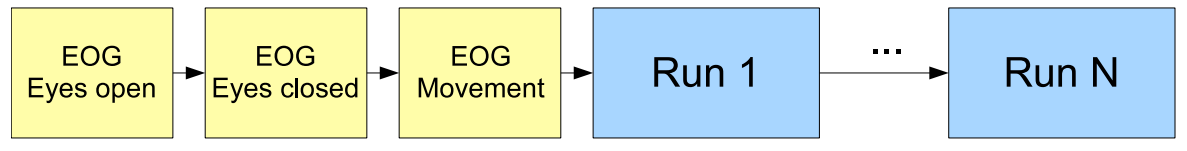
\includegraphics[width=0.8\textwidth]{2asession.png}
    \caption{2A session采集模式\cite{brunner2008bci}}
    \label{fig:2asession}
\end{figure}

在EOG记录之后,进行六次采集(run),在每个run中,各进行12次每类运动想象任务,这些任务的顺序是随机的,由此,一个run包含48次试验(trial),一个session包含288次试验(trial)。一个trial的流程如图~\ref{fig:2atrial}~所示,测试开始时(t=0s),一个十字图形出现在屏幕上,伴有简短的提示音;两秒后(t=2s),运动想象任务的指示箭头(分别指向左、右、下、上,对应左手、右手、双脚及舌头运动)出现在屏幕上,持续约1.25秒,每名被试进行运动想象任务直到十字图形消失(t=6s)。在这个过程中没有任何反馈。
\begin{figure}
    \centering
    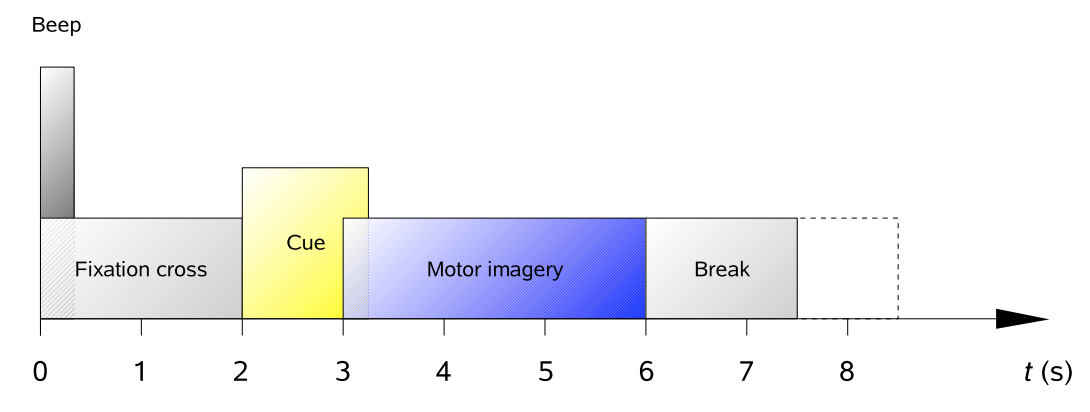
\includegraphics[width=0.8\textwidth]{2atrial.png}
    \caption{2A trial与无视觉反馈的2B trial的采集模式\cite{brunner2008bci,leeb2008bci}}
    \label{fig:2atrial}
\end{figure}

采集过程中,以250Hz进行EEG信号采样,并在0.5Hz至100Hz之间进行了带通滤波,放大器的灵敏度被设置为100\(\mu\)V,并使用了50Hz的陷波滤波器用以抑制线路噪声。头皮电极的位置按照国际10-20标准导联确定,共使用22个电极(通道),此外,还使用了3个不参与分类的EOG电极用以记录眼电信号。

在BCI领域,事件描述某一种波形或任务的起始点,数据上,事件表现为一个三元组:第一个元素以整数来描述的事件起始采样点;第二个元素对应当前事件来源的刺激通道(Stimulus Channel)的先前值(Previous Value),大多数情况下为0;第三个元素表示该事件的类型(Identify,id)。BCI Competition IV Dataset 2A数据集中共包含11类事件(Event),其中,与数据处理相关的事件如表~\ref{tab:2aevent}~所示,其中,拒绝试验是指由于质量欠佳或受试者未能有效完成而被专家标注出的试验数据。
\begin{table}[h]
    \centering
    \caption{2A事件类型列表}
    \label{tab:2aevent}
    \begin{tabularx}{0.8\textwidth}{>{\centering\arraybackslash\hsize=0.6\hsize}X >{\centering\arraybackslash\hsize=1.4\hsize}X}
    \toprule
    事件类型 & 描述 \\
    \midrule
    768 & trial开始  \\
    769 & 左手运动想象任务(class 1) \\
    770 & 右手运动想象任务(class 2) \\
    771 & 双脚运动想象任务(class 3) \\
    772 & 舌头运动想象任务(class 4) \\
    783 & 未知运动想象任务(测试集) \\
    1023 & 拒绝试验 \\
    \bottomrule
    \end{tabularx}
\end{table}

论文遵循BCI Competition竞赛设置,使用T文件为训练集,E文件为测试集,针对每名被试进行被试内实验和被试间实验。则在不剔除拒绝试验数据的情况下,每名被试的训练集和测试集切片数量分别为:288,288。

\paragraph{BCI Competition IV Dataset 2B}

BCI Competition IV Dataset 2B采取了类似2A数据集的采集方式,采集了9名被试的2类MI-EEG信号(左手、右手),每名被试在不同时间进行了五次session,数据以.gdf格式存储,每名被试有五个文件,例如,对于一号被试而言,B0101T.gdf、B0102T.gdf和B0103T.gdf为训练集,、B0104E.gdf和B0105E.gdf为测试集。其中,前两个文件不包含视觉反馈,后三个文件包含视觉反馈,即在试验过程中,通过屏幕上的笑脸图案对运动想象任务是否被正确执行予以反馈。无视觉反馈的session包含6次run,每个run包含20次trial(左手、右手各10次,随机排布),有视觉反馈的session包含4次run,每个run包含40次trial(左手、右手各20次,随机排布)。无视觉反馈的trial的采集模式与2A相同,如图~\ref{fig:2atrial}~所示。

BCI Competition IV Dataset 2B的事件类型与2A的事件类型相似,但不包含双脚和舌头运动想象任务。此外,不同于2A数据集的22个电极,2B数据集仅使用3个电极记录数据。

为了保证实验数据只涉及运动想象,而不涉及视觉反馈,论文选择无视觉反馈的两个session分别作为训练集和测试集,则在不剔除拒绝试验数据的情况下,每名被试的训练集和测试集切片数量分别为:120,120。

综上所述,论文所使用的数据的信息如表~\ref{tab:dataset}~所示。
\begin{table}[ht]
    \centering
    \caption{数据集信息}
    \label{tab:dataset}
    \begin{tabularx}{\textwidth}{CCC}
      \toprule
      数据集 & BCI IV 2A & BCI IV 2B \\
      \midrule
      被试数量 & 9 & 9 \\
      类别数量 & 4 & 2 \\
      通道数量 & 22 & 3 \\
      频率范围 & 0.5-100Hz & 0.5-100Hz \\
      采样频率 & 250Hz & 250Hz \\
      训练集数据量 & 288(每被试) & 120(每被试) \\
      测试集数据量 & 288(每被试) & 120(每被试) \\
      \bottomrule
    \end{tabularx}
\end{table}

\subsection{数据预处理}

EEG信号具有低信噪比、非平稳、空间变异性等特性,并且通常具有较小规模的数据集,一般来说,对数据进行一定的预处理有助于后续分类任务。然而,论文基于端到端网络的思想构建模型,因此尽可能地对预处理操作进行削减。论文进行的数据预处理方法如下:

\paragraph{数据提取与切片}

MI-EEG原始信号储存在.gdf格式的文件中,除目标脑电信号之外,原始文件还包括EOG信号、间隙缺失值、与运动想象任务不直接相关的事件等。因此,在提取数据时,有必要进行一定的处理:

首先,剔除EOG通道数据,仅保留EEG通道数据,对于用于分隔run的缺失值(编码为非数字,NaN),使用对应通道的均值替代,以确保数据的连续性和完整性;

其次,对与运动想象任务直接相关的事件进行筛选和提取,并对相关时段进行切分。对于BCI Competition IV的2A/2B数据集,直接相关事件为四类/二类运动想象任务事件,并由提示信号(Cue)标识任务的开始,论文对连续数据进行切片,提取从Cue出现后的第1秒至第4秒(trial周期的第3秒至第6秒)的数据段,作为事件对应的运动想象任务持续期间产生的EEG信号,在后续加以分析。对于采样率为250Hz的数据集而言,3秒的数据区间将包含750个采样点。

需要说明的是,论文在数据提取过程中并未对拒绝试验进行剔除,同时未使用滤波器对EEG信号的频率进行过滤,以对真实应用情境中可能出现的多样化数据表现进行模拟,对模型自主识别各种频率成分并提取有效特征的能力进行评估。

\paragraph{标准化}

归一化操作的目的在于对数据的特征尺度进行统一,从而消除奇异数据导致的不良影响,提高模型的训练效率和稳定性。EEG信号常用的归一化方法有Z-score标准化、最大最小值归一化等。

Z-score标准化的操作过程如公式~\ref{eq:z-score}~所示,其中,x为原始数据,\(\mu\)表示数据的均值,\(\sigma\)表示数据的标准差,Z-score通过均值和标准差对数据进行操作,使得处理后的数据符合均值为0,方差为1的标准正态分布。
\begin{equation}
    x=\frac{x-\mu}{\sigma}
    \label{eq:z-score}
\end{equation}

最大最小值归一化的操作过程如公式~\ref{eq:maxmin}~所示,其是一种线性变换操作,将数据映射至\([0,\,1]\)区间,其中,\(X\)为一组通道数据。最大最小值归一化计算简单,但对具有波动性的EEG信号而言,将数据缩放至\([0,\,1]\)区间容易导致数据特征的损失。
\begin{equation}
    x=\frac{x-min(X)}{max(X)-min(X)}
    \label{eq:maxmin}
\end{equation}

因此,为了尽可能保留EEG信号的特征,论文采用Z-Score标准化方法对EEG信号进行处理,以提高模型训练的速度和稳定性。

\paragraph{数据增强}

MI-EEG信号通常具有较小规模的数据集,因此,通过一定的数据增强操作扩大数据规模,有助于提升网络训练效果,防止过拟合现象的发生。然而,在BCI系统的实际应用中,数据增强操作可能会导致训练阶段数据处理压力的增长,因此,在论文中,数据增强是一项可选操作,其目的在于提高模型分类精度,论文将分别使用进行数据增强和不进行数据增强的数据集进行训练。

EEG信号的数据增强方法主要有以下几种:

(1) 添加随机噪声:在EEG信号上叠加高斯白噪声、有色噪声等不同类型的噪声,模拟真实环境中的噪声干扰,能够提升模型的抗噪性和鲁棒性;

(2) 滑动窗口:设定时间滑动窗口的长度小于运动想象任务持续的时间长度,将滑动窗口内的数据视作一次事件,通过滑动窗口对数据进行切片,有助于模型学习EEG信号随时间变化的特征;

(3) 频率混叠:在保持EEG信号特性的前提下,将多种不同频率成分进行混叠,使得模型能够学习更广泛的频率特征;

(4) 生成对抗网络(Generative Adversarial Network, GAN):基于GAN生成拟真的EEG数据,对原始数据进行扩充。

由于在预处理阶段没有采取频率滤波的操作,论文采取频率混叠的方式对EEG信号进行增强,从而加强模型识别不同频率成分的能力。具体来说,

\begin{algorithm}[H]\label{alg:aug}
    \caption{数据增强算法}
    \SetAlgoLined
    
    \KwData{A set $E_o = \{e_1, e_2, ..., e_n\}$ and a similarity threshold $\theta$.}
    \KwResult{The Uniqueness-Index $u(E_o)$ of the set $E_o$.}
    
    $counter \leftarrow 0$\;
    
    \For{each item $e_i \in E_o$}{
        \For{each item $e_j \in E_o$ where $j \neq i$}{
            $similarity \leftarrow \text{CosSim}(v_i, v_j)$\;
            \If{$similarity < \theta$}{
                $counter \leftarrow counter + 1$\;
            }
        }
    }
    
    $u(E_o) \leftarrow \frac{2 \times C}{n \times (n - 1)}$\;
    
    \Return{$u(E_o)$}\;
\end{algorithm}

\subsection{实验准备}

\paragraph{评价指标}

\paragraph{损失函数}

\paragraph{参数配置}

\section{实验设计}

\subsection{DIS-Net实验设计}

为了确定模型架构的最佳设置,本节对DIS-Net构建过程中不同的模型架构进行实验,从而逐步构建起性能最优的模型。

\paragraph{Inception模块引入空间卷积层的方式}

在DI-Net中,空间卷积层有两种不同的方式融入基于Inception改进的时间卷积层之后,一种是在每个Inception模块内部的分支结构上增加空间卷积层,另一种则是在整个Inception模块之后附加空间卷积层。图~\ref{fig:ts-incep}~展示了这两种引入方式的区别,将这两种方式分别称为分支内融合(Inception-In)和模块后融合(Inception-After),需要说明的是,图中省略了网络的其他结构,如瓶颈层等,以尽可能简洁地展现不同引入方式的差异。其中,\(s\_kernel\)表示空间卷积核,\(t\_kernel_i\)表示第\(i\)个分支的时间卷积核。
\begin{figure}
  \centering
  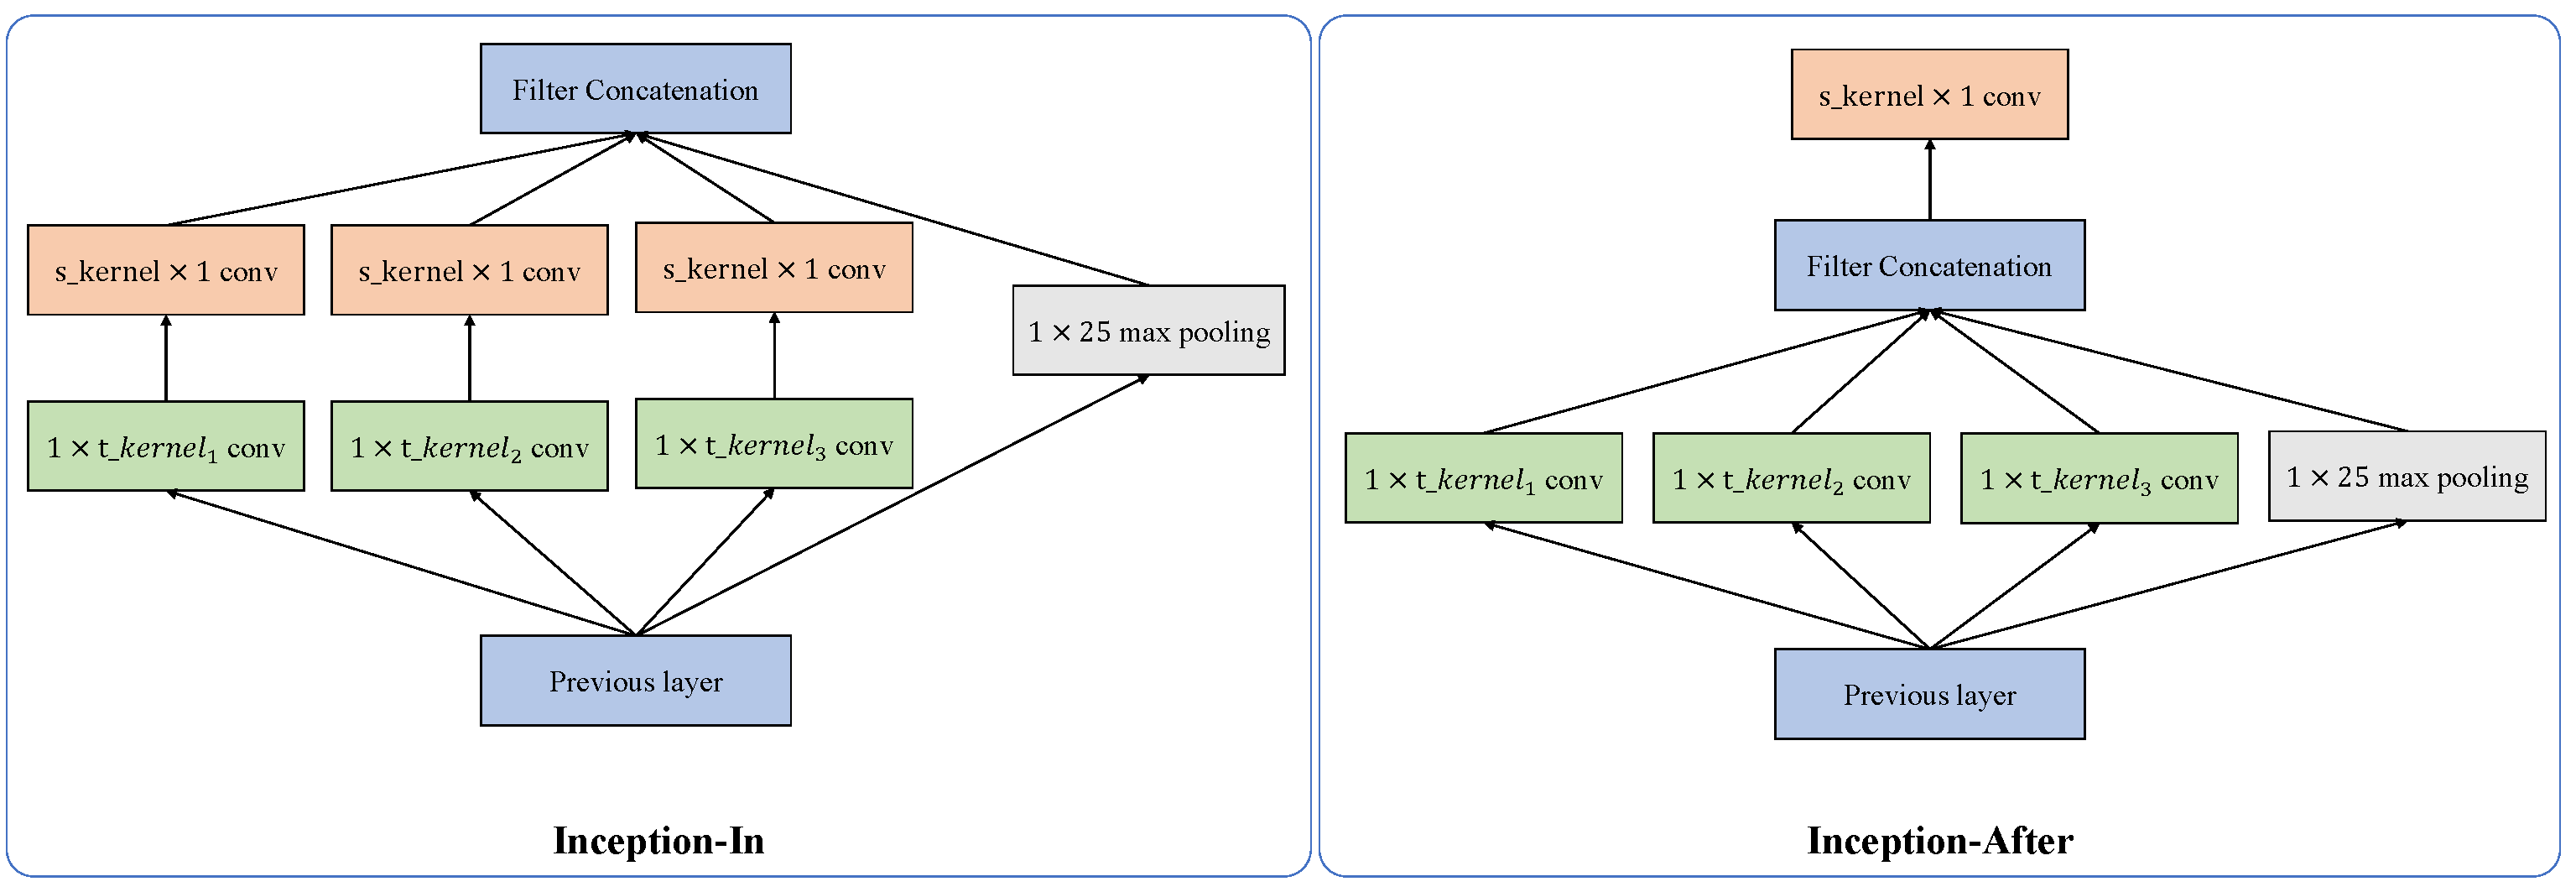
\includegraphics[width=\textwidth]{ts-incepv3.pdf}
  \caption{Inception模块引入空间卷积层的方式}
  \label{fig:ts-incep}
\end{figure}

为了比较Inception-In与Inception-After的性能差异,论文在BCI Competition IV Dataset 2A数据集上设计实验进行对比。在实验设置阶段,固定了Inception模块的层次数量、分支数量等参数,实验结果如表~\ref{tab:ts-inception}~所示。在此,重点关注两项评价指标——准确率(Accuracy, ACC)和Kappa一致性系数(Kappa),这两项指标均基于数据集中九位被试的平均表现。实验结果显示,Inception-After方式在准确率和一致性系数上均表现更优。这一优势可能源自两方面的原因:一方面,虽然Inception-In模式借鉴了FBCSP算法的分频段处理思路,但在Inception分支内部直接进行空间特征提取的过程中,损失了部分空间全局信息;另一方面,Inception-In结构具有相对更大的参数规模,这可能导致模型在有限样本条件下更容易出现过拟合现象。基于以上分析和实验验证,论文选择以Inception-After的方式布局时间卷积层与空间卷积层。
\begin{table}[ht]
  \centering
  \caption{Inception-In、Inception-After实验结果对比}
  \label{tab:ts-inception}
  \begin{tabularx}{\textwidth}{CCC}
    \toprule
    Models & ACC(\%) & Kappa \\
    \midrule
    Inception-In & 63.31 & 0.51 \\
    Inception-After & \textbf{75.35} & \textbf{0.70} \\
    \bottomrule
  \end{tabularx}
\end{table}

\paragraph{svSE模块的引入方式}

DIS-Net中,由于DI-Net的特征提取过程分为时间卷积和空间卷积两个阶段,svSE模块可采取以下三种引入方式:其一是在时间卷积层后引入;其二是在空间卷积层后引入;其三是同时在时间卷积层和空间卷积层之后引入。图~\ref{fig:att-Base}~展示了这三种引入svSE模块的方式,从左至右分别是时间卷积层后引入svSE模块、空间卷积层后引入svSE模块,以及在时间卷积和空间卷积层后均引入svSE模块。将这三种引入方式对应的模型分别简称为S-Temporal-Net、S-Spatial-Net、S-TS-Net。
\begin{figure}
  \centering
  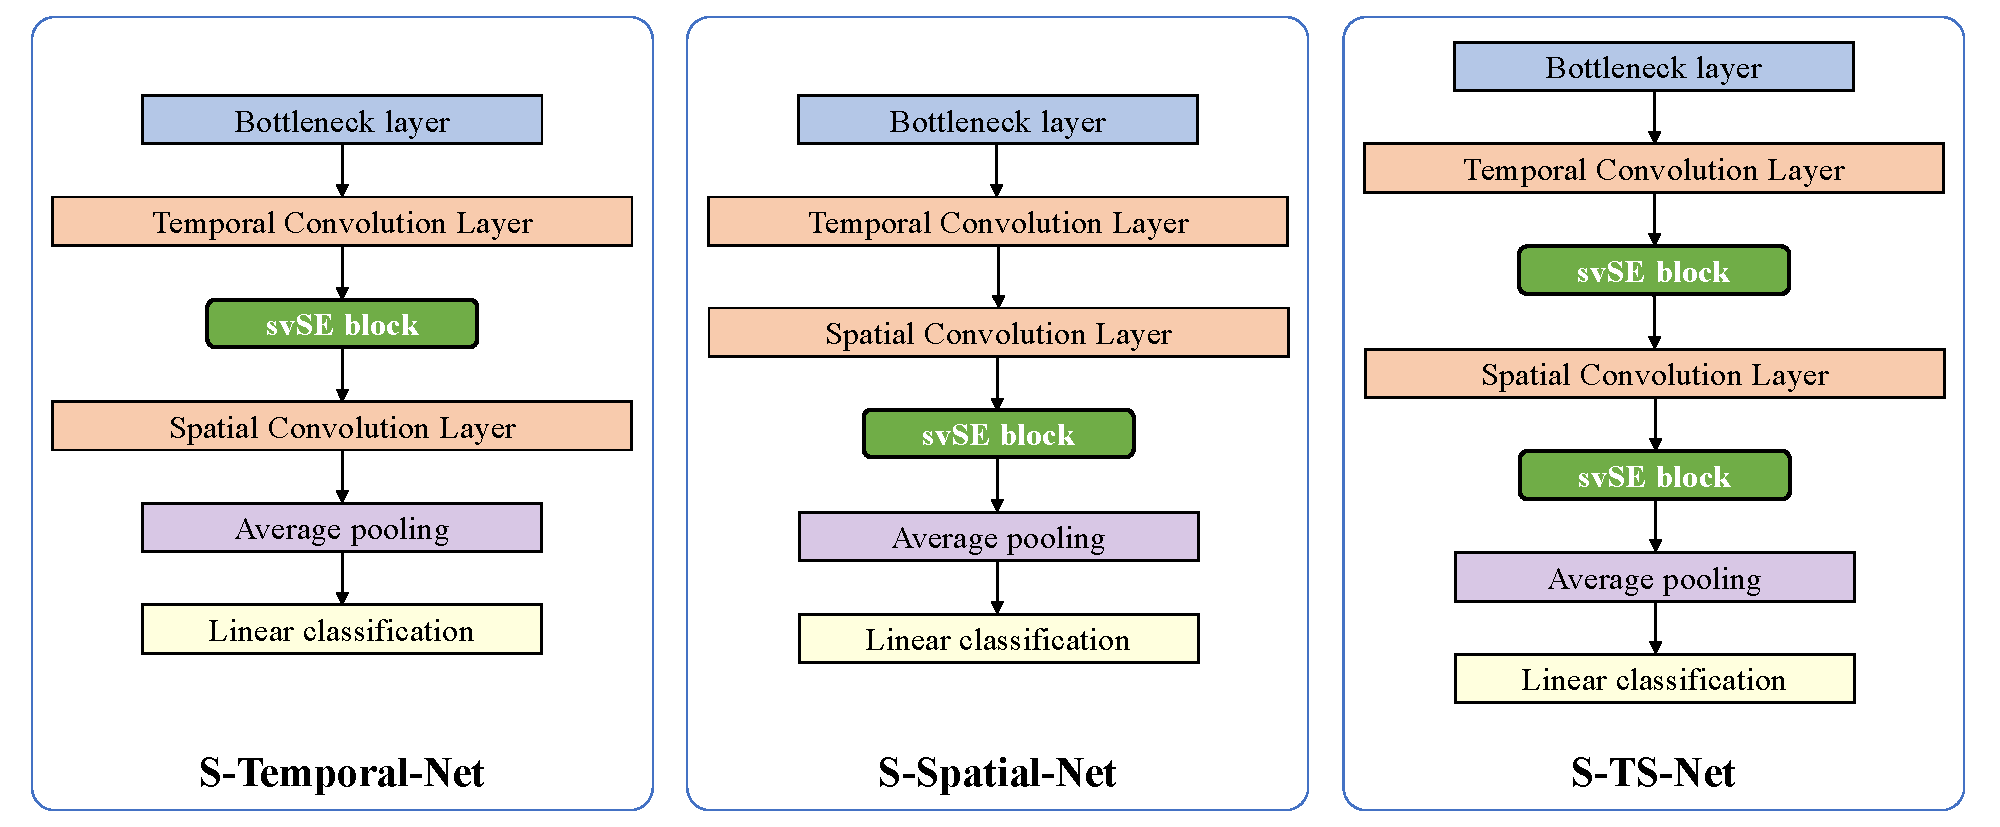
\includegraphics[width=\textwidth]{att-Basev2.pdf}
  \caption{DI-Net引入注意力模块的方式}
  \label{fig:att-Base}
\end{figure}

表~\ref{tab:svSE-BaseNet}~展示了S-Temporal-Net、S-Spatial-Net、S-TS-Net三种模型在BCI Competition IV Dataset 2A\cite{tangermann2012review}数据集上的对比实验结果。实验采用固定的参数,表格中展示的准确率(Accuracy,ACC)和Kappa一致性系数(Kappa)指标为数据集中九位被试的平均表现,标准差(Standard Deviation,SD)则为准确率的标准差。从准确率和一致性分析,S-ST-Net模型的效果优于其他两种模型,与经验相符。此外,S-Temporal-Net模型的效果优于S-Spatial-Net模型,其原因可能在于,空间卷积层沿通道维度的卷积使得数据损失了部分特征,进而减弱了svSE模块提取关键特征权重的能力,而时间卷积层保留了大部分深度信息和通道信息,因此,在时间卷积层之后加入svSE模块能够帮助模型更好地捕捉深度和空间的特征。从标准差分析,S-TS-Net模型的准确率波动幅度较小,对不同被试的MI-EEG分类效果相对均衡,另外两种模型在不同被试间的分类精度则存在较为明显的差异。实验数据显示,S-TS-Net模型取得了更好的效果,因此,论文采用同时在时间卷积层和空间卷积层之后引入svSE模块的方式,将这种结构的模型称为DIS-Net。
\begin{table}[ht]
    \centering
    \caption{svSE模块引入位置对比}
    \label{tab:svSE-BaseNet}
    \begin{tabularx}{\textwidth}{CCCC}
        \toprule
        Models & ACC(\%) & Kappa & SD \\
        \midrule
        S-Temporal-Net & 78.09 & 0.71 & 10.38 \\
        S-Spatial-Net & 77.16 & 0.69 & 10.24 \\
        S-TS-Net & \textbf{78.55} & \textbf{0.71} & \textbf{9.46} \\
        \bottomrule
    \end{tabularx}
\end{table}

\subsection{LS-Net实验设计}

\subsection{各模块消融实验}

\subsection{超参数优化实验}

\subsection{BCI Competition IV Dataset 2A数据集上的对比试验}

\subsection{BCI Competition IV Dataset 2B数据集上的对比试验}

\section{本章小结}


GhostNet的优势在于其Ghost模块设计,该模块凭借对特征图间内在相似性的有效利用,实现了低成本的特征转换操作,同时,GhostNet中同样使用了权重参数 \(ratio\),用以控制经由廉价线性转换进行操作的特征图的比例,其中,使用普通卷积的分支其特征图数量为\(D_{out} \times ratio\),其中,\(D_{out}\)为输出特征图数量,使用深度卷积的分支其特征图数量为\(D_{out}-D_{out} \times ratio\)。

然而,Ghost模块在运用线性变换与传统卷积相结合的方式来产生新特征图的过程中,尚存在一定的局限性,即生成的特征图之间交互作用不充分。鉴于此,论文进一步改良了Ghost模块,引入了通道混洗机制,构建出SG模块(Shuffle Ghost Module)。SG模块的结构如图~\ref{fig:sg}~所示,通过通道混洗机制增强不同特征图之间的相互作用,进而提升网络的整体表现力和特征学习能力,图中的DW Conv指深度卷积。此外,SG模块采用与GAS模块相同的方式对Ghost模块内部的卷积核大小进行了修改,并加入了批归一化和GELU激活函数。
\begin{figure}
    \centering
    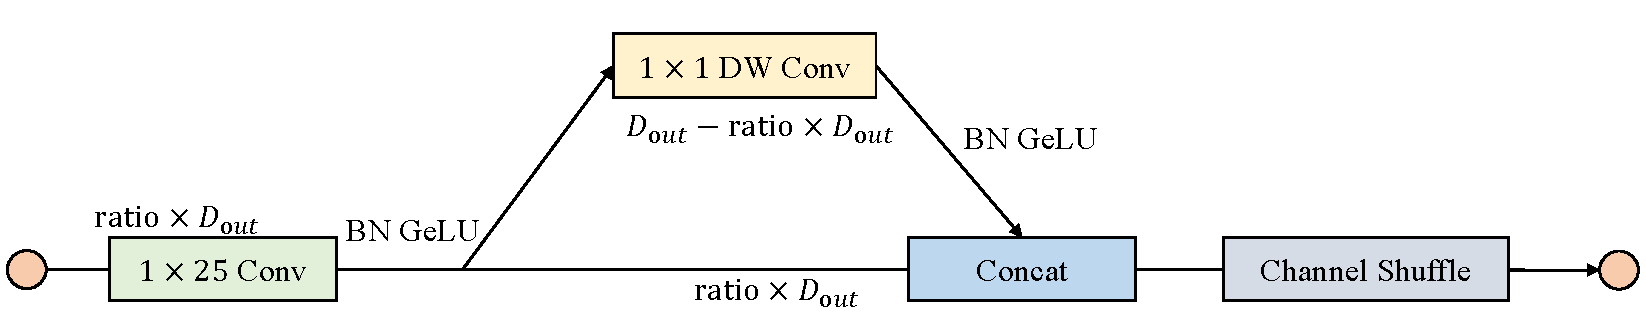
\includegraphics[width=\textwidth]{SG.pdf}
    \caption{SG模块结构}
    \label{fig:sg}
\end{figure}

为了验证更适合的轻量化卷积模块,论文在BCI Competition IV Dataset 2A数据集上进行了实验验证。由于轻量化卷积主要针对密集连接进行改进,实验使用DI-Net,并固定了Inception层数、密集连接层数、学习率、\(ratio\)等超参数。表展示了GAS/SAS、SG和原始(Origin)模块的对比实验结果,其指标为参数量(Parameters)、浮点运算数(Floating Point Operations,FLOPs)和准确率(Accuracy,Acc),其中,准确率为九位被试的平均值。
\begin{table}[ht]
    \centering
    \caption{轻量化卷积模块实验结果对比}
    \label{tab:lite}
    \begin{tabularx}{\textwidth}{CCCC}
      \toprule
      Models & Paramters & FLOPs & ACC(\%) \\
      \midrule
      GAS/SAS(0.5) & 7.31K & 130.37M & 74.61\\
      GAS/SAS(0.4) & 7.83K & 143.44M & 73.80\\
      GAS/SAS(0.6) & \textbf{6.80K} & \textbf{117.75M} & \textbf{74.61}\\
      SG(0.5) & 7.27K & 129.93M & 73.26\\
      SG(0.4) & 7.67K & 139.73M & 72.22\\
      SG(0.6) & 7.27K & 129.93M & 73.00\\
      Origin & 29.99K & 690.37M & \textbf{75.62}\\
      \bottomrule
    \end{tabularx}
\end{table}